\section{Transition from RNN to Transformers } 
In this chapter, we will explore the significant transition from Recurrent Neural Networks (RNNs) to Transformers in the field of Natural Language Processing (NLP). A pivotal milestone in this journey, as discussed in Chapter 7, was the introduction of the attention mechanism in sequential models. Following this development, the NLP community began questioning whether RNNs were indeed the optimal choice for modeling sequences or if alternative approaches could yield better results.

The initial indication of this paradigm shift emerged with the development of CNN-like architectures for sequence processing. Traditionally, CNNs and RNNs have been distinguished by their input characteristics, with CNNs typically handling fixed-length inputs and RNNs accommodating variable-length inputs. However, since an image can be viewed as a two-dimensional input patches sequence, it becomes feasible to apply CNNs to sequence modeling tasks.

CNNs deal with sequence modeling differently from RNNs. Instead of preserving the order of the sequence, CNNs adopt a bottom-up approach, extracting features \textbf{hierarchically} from local regions of the input. While this departure from sequential processing might seem unconventional, CNNs offer several advantages. Firstly, the processing of each element in the sequence occurs \textbf{uniformly across the entire input}, facilitated by the shared parameters within each layer. This uniform processing contributes to the homogeneity of the model's operations. Additionally, CNNs exhibit enhanced scalability, particularly when accelerated by \textbf{GPU computing}, due to their inherent parallelism.

By leveraging CNNs for sequence modeling, practitioners can benefit from their efficiency in capturing \textbf{local patterns} and their ability to exploit \textbf{parallel computation}, making them a compelling alternative to traditional RNN architectures. This shift laid the groundwork for subsequent advancements in sequence modeling, ultimately leading to the emergence of Transformer architectures (refining and extend these benefits in a distinct design).

To understand how a Convolutional Neural Network extracts context from an input sequence to produce a translation, we first need to delve into a crucial concept: \textbf{Dilation}, which refers to the spacing between the elements (or receptive fields) of a filter as it moves across the input sequence. 

\begin{figure}[!htbp]
    \centering
    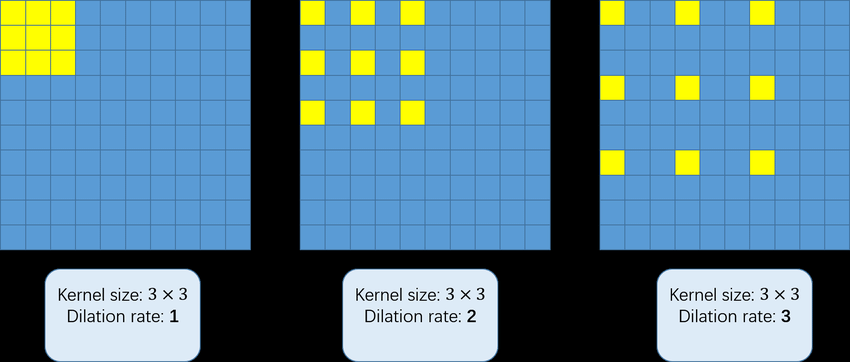
\includegraphics[width=0.85\linewidth]{tikz/chapter8 - Dilation.png}
    \caption{{\color{red}\colorbox{pink}{Tikz TO-DO}} Example of Three Different Dilation Rate}
\end{figure}

In Chapter 5, we introduced CNN architecture, focusing on the traditional convolutions, which have a dilation rate of 1, meaning that the kernel considers adjacent pixels. 

Unlike traditional convolutions, dilated convolutions introduce gaps between the elements of the filter. This allows the network to capture information over larger spans of the input sequence. For instance, with a dilation rate of 2 (skipping 1 pixel) or 3 (skipping 2 pixels), as shown in the figure above, we achieve the same number of features in the next layer without changing the kernel size. This approach extends the receptive field of the convolutional filter, enabling it to incorporate more context from the input data while maintaining the computational efficiency of the original kernel size.


\section{Temporal Convolutional Network}

Convolutional Sequence Model, also called \textbf{Temporal Convolutional Network} (TCN), was the first architecture to apply a CNN to sequence processing. It was introduced in the work \href{https://arxiv.org/pdf/1803.01271}{"An Empirical Evaluation of Generic Convolutional and Recurrent Networks for Sequence Modeling" (Bai et al.)} and marked the shift from RNN to CNN for sequence input problems.

TCNs are distinguished by two main features:
\begin{itemize}
    \item \textbf{Sequence Length Preservation}: The architecture of TCNs can take a sequence of any length and map the input to an output sequence of the same length.
    \item \textbf{Causality in Convolutions}: The convolutions used in the architecture are causal, ensuring that there is no loss of information from the future to the past.
\end{itemize}

To achieve sequence length preservation, TCNs use a 1D fully convolutional network (FCN) architecture, where each hidden layer has the same length as the input layer. Length padding ($\text{kernel size} - 1$) is added to preserve the length of subsequent layers, ensuring that they match the length of the previous layers.

To maintain causality, TCNs employ \textbf{dilated causal convolution}, which is a 1D convolution operation in which the output at time $t$ is computed using specific elements of the input positions of the previous level, determined by the dilation rate. This method ensures that each output depends only on specific past inputs, respecting the causality constraint. This convolution operation is crucial for capturing temporal dependencies in sequential data, as it ensures that predictions are based only on past information, avoiding any "loss" of future information in past data. \textbf{Residual connections} are also used to enhance the learning process.

To put it simply, a TCN can be viewed as a combination of a 1D FCN and dilated causal convolution layers. In addition, the model uses the ReLU activation function and dropout as regularization techniques. An additional trick used is the \textbf{weight normalization block}, which normalizes the vector of weights, accelerating convergence without introducing dependencies between examples in a minibatch, which is the reason for using it.

For a better understanding see this explanatory diagram:

\begin{figure}[!htbp]
    \centering
    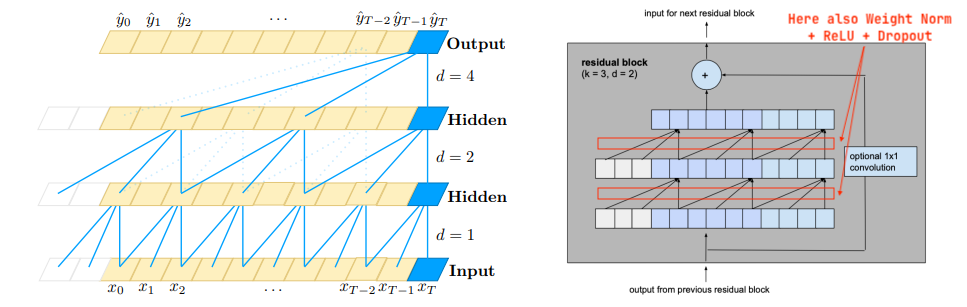
\includegraphics[width=0.95\linewidth]{tikz/chapter8 - Temporal Convolutional Network.png}
    \caption{{\color{red}\colorbox{pink}{Tikz TO-DO (on the right, but merge the one on the left)}} A global overview of Dilated Causal Convolution.}
\end{figure}

The architecture differs significantly from standard CNNs because the output of each hidden layer is obtained using dilation (1, 2, 4) and kernels of size 3. The most notable change is the causal effect: the CNN has been adapted to predict tokens sequentially. For example, the output $y_t$ is predicted after $y_{t-1}$ using only a "shifted" number of features from the previous level, i.e. $x_t, x_{t-4}, x_{t-8}$.


\section{Convolutional Seq2Seq learning}
In \href{https://arxiv.org/pdf/1705.03122}{"Convolutional Sequence to Sequence Learning" (Auli et al.)} Google's Seq2Seq learning model is adopted and CNN-based approach is introduced. In this work, the task is to translate a sentence from German to English.

In the original architecture (RNN with Attention), the encoder consists of a bidirectional LSTM. The output of this bidirectional LSTM is concatenated to form the input for subsequent layers. This concatenated output is then used to construct a soft attention mechanism, which captures important relationships within the input sequence. Next, the decoder provides English translation using the latent representations associated with the concatenated output and the attention mechanism.

In this work, researchers replaced the bidirectional LSTM in the encoder with a Temporal Convolutional Neural Network (TCN), which produces latent representations used for attention computation. In addition, the decoder was also transformed to a CNN-based architecture. In both cases, encoder and decoder, Gated Linear Units and residual connections are used.

\begin{figure}[!htbp]
    \centering
    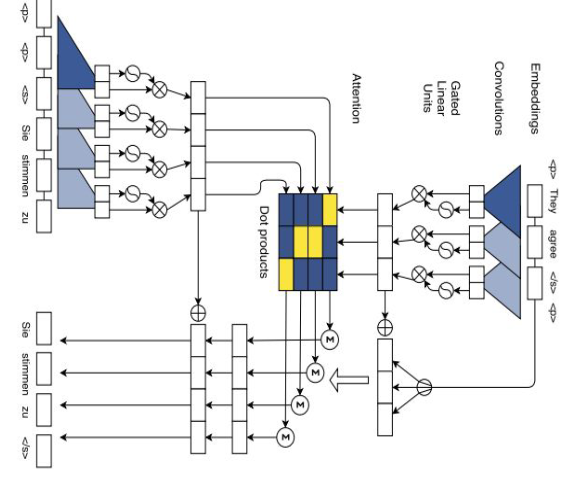
\includegraphics[width=0.6\linewidth]{tikz/chapter8 - Convolutional Seq2Seq.png}
    \caption{{\color{red}\colorbox{pink}{Tikz TO-DO}} Convolutional Seq2Seq Architecture}
\end{figure}

The CNN-based decoder improves training efficiency by exploiting parallel computing capabilities. Both the encoder and decoder consist of 15 levels each.

\section{Attention is All You Need}

Transformers are a novel neural network architecture introduced the paper \href{https://arxiv.org/pdf/1706.03762}{"Attention Is All You Need" (Vaswani et al.)}. They are based on a \textbf{self-attention mechanism}, forming the backbone of neural machine translation architectures that use fully connected (FC) layers and attention.

Compared to recurrent or convolutional architectures, Transformers are more efficient and easier to parallelize. This characteristic makes them faster to train and capable of handling larger datasets effectively.

The classical Transformer architecture is composed of two main components: the encoder and the decoder.
\begin{itemize}
    \item \textbf{Encoder}: The encoder processes the entire input sequence at once and outputs an encoded sequence of the same length. Each input word is transformed into a high-dimensional vector representation.
    
    \item \textbf{Decoder}: The decoder generates the output sequence one word at a time. It is conditioned on the encoded sequence from the encoder and the previously predicted words. This ensures that the decoder takes into account both the context provided by the encoder and the sequence of words generated so far.
\end{itemize}


\subsection{But what is Self-Attention?}

Self-Attention is a mechanism that captures the context of other words relevant to the one we are currently processing. This makes it possible to create long-range weighted dependencies between word tokens in language models. In practice, it allows the model to focus on words that are important for understanding the meaning of a word at a given position in the sentence.

To calculate self-attention, we start by creating three vectors from the embeddings: \textbf{query ($Q$)}, \textbf{key ($K$)} and \textbf{value ($V$)}. These vectors are obtained by \textbf{multiplying the word embeddings} ($X$) \textbf{by three different weight matrices} ($W^Q$, $W^K$ and $W^V$) learned during the training process. Here's the meaning of these vectors:
\begin{itemize}
    \item $Q$: the query represents the current word for which we are searching for relevant words.
    \item $K$: the key represents the potentially relevant words.
    \item $V$: the value represents the content of the relevant words.
\end{itemize}

The self-attention formula is as follows:

$$
    \text{Attention}(Q,K,V) = \text{softmax}\left(\frac{QK^T}{\sqrt{d_k}}\right)V
$$

The scalar product between query and key ($QK^T$) is called \textbf{score} and measures how similar two words are. In other words, it indicates \textbf{how much we need to focus on other words in the input sentence} while processing a specific word. To obtain stable scores, we divide the scalar product between the query and the keys by the square root of the size of the keys (\(d_k\)) and apply softmax. The word in that position will have the highest softmax score, but \textbf{it may also pay attention to another relevant word}. We multiply each value ($V$) by the softmax score, keeping the values of important words and reducing those of irrelevant words. We then sum these weighted values to get the self-attention output for that position ($Z$). Graphically:

\begin{figure}[!htbp]
    \centering
    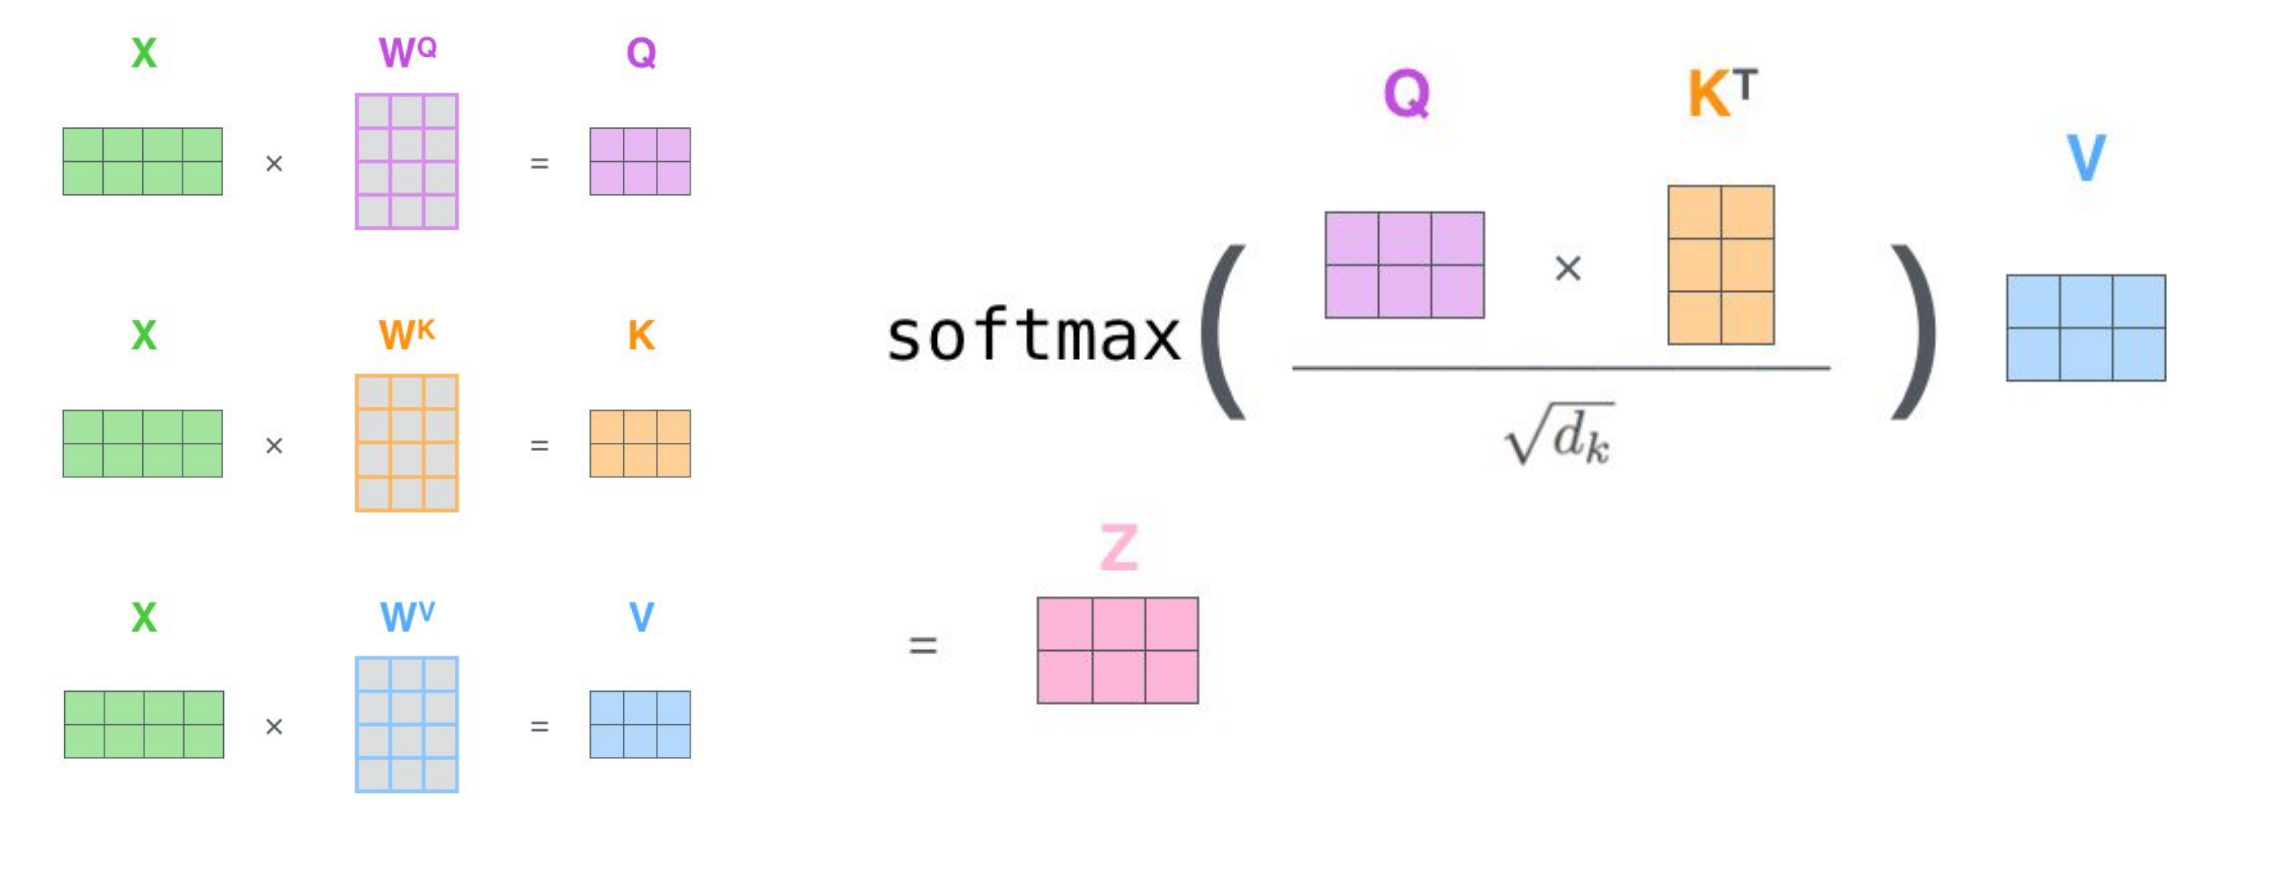
\includegraphics[width=0.8\linewidth]{tikz/chapter8 - Self-Attention Calculation.png}
    \caption{{\color{red}\colorbox{pink}{Tikz TO-DO}} Self-Attention Calculation}
\end{figure}

One thing that is important is that soft attention is differentiable, making it easy to train the model by backpropagation.


\subsection{Multi-Head Attention}
In transformers, we use \textbf{multi-head attention} to improve the model's ability to focus on different positions in the sentence and provide the attention level with more "subspaces of representation". For example, some heads may focus on words nearby, while others may focus on words far away in the text. This allows the model to capture a wider range of information.

But how does it work? In multi-head attention, vectors of input embeddings are divided into \textbf{several separate "heads"}. Usually in the classical Transformer, this number is 8. Each head of multi-head attention operates on the linear projections we have already seen: query, key and value. After calculating the attention for each head, the results are \textbf{concatenated and multiplied by an additional weight matrix} to produce the final attention level output.

\begin{figure}[!htbp]
    \centering
    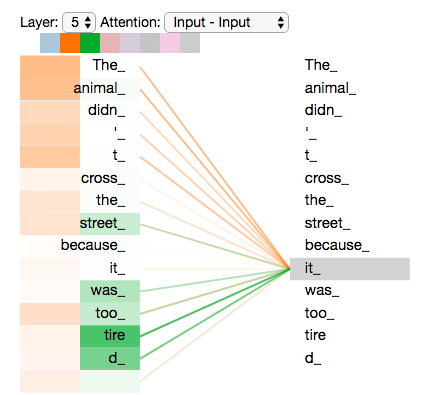
\includegraphics[width=0.5\linewidth]{tikz/chapter8 - Multi Head Self-Attention.png}
    \caption{{\color{red}\colorbox{pink}{Tikz TO-DO}} Multi Head Self-Attention}
\end{figure}

The image provided shows a visualization of the outputs using two heads. We can see that if the query word is "it", the first head focuses more on the words "the animal", while the second head focuses on the word "tired". As a result, the final context representation takes into account all the words "the", "animal", and "tired", providing a richer and more accurate representation than traditional methods.


\subsection{Positional Encoding}

Before passing the embeddings as input to the Encoder and Decoder, it is critical to add information regarding the position of each word. Unlike other models, such as recurrent neural networks, the Transformer has no intrinsic sense of the order or position of words within a sentence. To compensate for this lack, we use \textbf{positional encoding}.

When we combine word embeddings with positional encoding in the context of Transformer models, we obtain "\textbf{time-signal embeddings}". This means that each embedding vector not only represents the meaning of the word, but also includes a component that indicates its relative position in the input sequence. 

One of the common techniques for positional encoding is the use of \textbf{sinusoidal functions}, which allow different positions in the embedding vector to be represented. This method helps to maintain consistency of positional information despite arbitrary word order, which is essential for the proper functioning of the Transformer.


\subsection{The Architecture}

The architecture includes all the elements explained so far. Before moving to the encoder and decoder, embeddings are computed with positional encoding added.

The Encoder consists mainly of two modules: the \textbf{Multi-Head Attention} and the \textbf{Feed-Forward Network}, which processes the output vectors of the multi-head attention. This layer is independent along different paths, enabling parallel execution.

The Decoder, in contrast, consists of three separate modules: the \textbf{Multi-Head Attention}, the \textbf{Masked Multi-Head Attention}, and the \textbf{Feed-Forward Network}. The Masked Multi-Head Attention is used because it is critical to \textbf{prevent future positions in the sequence from affecting subsequent ones}, thus allowing the Decoder to examine only earlier information. The additional module of Attention Multi-Head is used to operate on the outputs of the Encoder stack, allowing the Decoder to focus on different parts of the Encoder input, improving the model's ability to capture information relevant to output generation.

\begin{figure}[!htbp]
    \centering
    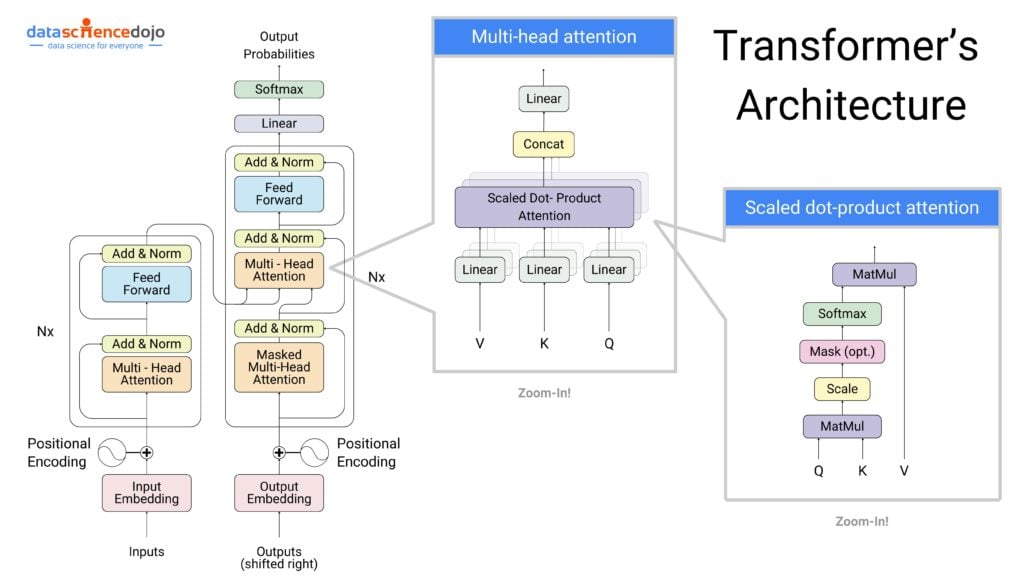
\includegraphics[width=0.85\linewidth]{tikz/chapter8 - TRANSFORMERS.jpg}
    \caption{{\color{red}\colorbox{pink}{Tikz TO-DO}} Transformer Architecture}
\end{figure}

In both the Decoder and the Encoder, \textbf{Residual Connections} and \textbf{Layer Normalizations} are used to provide greater stability during training and to facilitate the flow of gradients through the various layers of the architecture.

In the visual representation, it is emphasized with a kind of magnifying glass how a multi-head attention module is structured, which in turn includes numerous self-attention modules for each of its heads.

In conclusion, transformers offer significant advantages, such as \textbf{efficient parallel computations} and improved handling of long sequences compared to previous architectures like RNNs and CNNs. Moreover, the paradigm of \textbf{pre-training language models on large-scale datasets}, followed by fine-tuning for specific tasks, has transformed natural language processing.

After the advent of transformers, the community began exploring models that utilize \textbf{either the encoder or decoder independently}. The first category leverages output hidden states, which can serve as features in broader models designed for diverse tasks (e.g., BERT). The second category, specifically designed for text generation, proves highly effective for applications such as machine translation or summarization (e.g., GPT series).

\begin{figure}[!htbp]
    \centering
    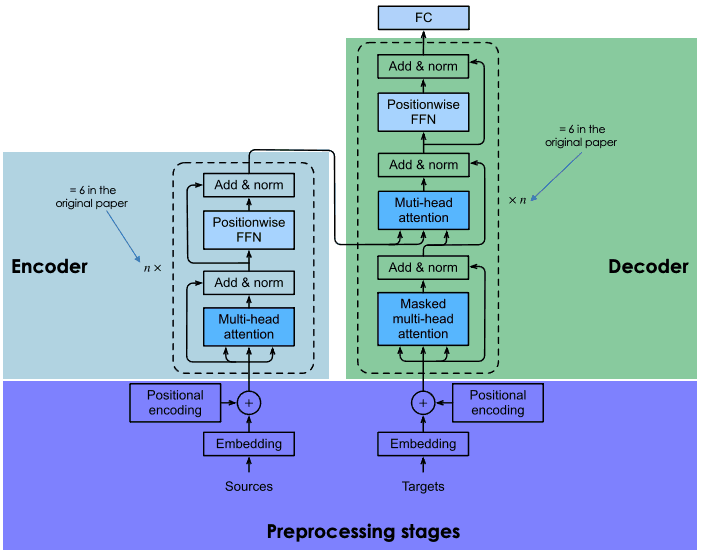
\includegraphics[width=0.85\linewidth]{tikz/AGGIUNGI A IMMAGINE TRANSFORMERS.png}
    \caption{{\color{red}\colorbox{pink}{Tikz TO-DO: Aggiungere Aree + numero a immagine transformers}}}
\end{figure}

\section{Vision Transformer (ViT)}


In the context of convolutional neural networks, a significant limitation has been the concept of \textbf{receptive field}, which is related to the size of the convolutional kernel. This limitation has affected the ability of CNNs to capture complex, long-range relationships within images.

Visual Transformer, introduced in \href{https://arxiv.org/pdf/2010.11929}{"An Image is Worth 16x16 Words: Transformers for Image Recognition at Scale" (Dosovitskiy et al.)}, marked a fundamental step in the evolution of neural networks for computer vision. ViT extended the capability of convolutions by applying the concept of self-attention to images as well, thus transferring the Transformer model from the field of natural language processing (NLP) to the field of computer vision, dealing with three-dimensional rather than two-dimensional data.

Self-attention is a mechanism for constructing \textbf{learnable long-range semantic relations}. In this case, the concept is transformed into \textbf{learning the relationships between pixels in fixed areas of the image}. The main difference of self-attention from NLP is that, in computer vision, it is used to model self-similarity within images. For example, if there are two cars in the background of an image, the areas that include these objects will be detected as similar. Therefore, to pass an input image to the encoder, it is divided into "\textbf{patches}", deciding in advance the number of divisions.

\begin{figure}[H]
    \centering
    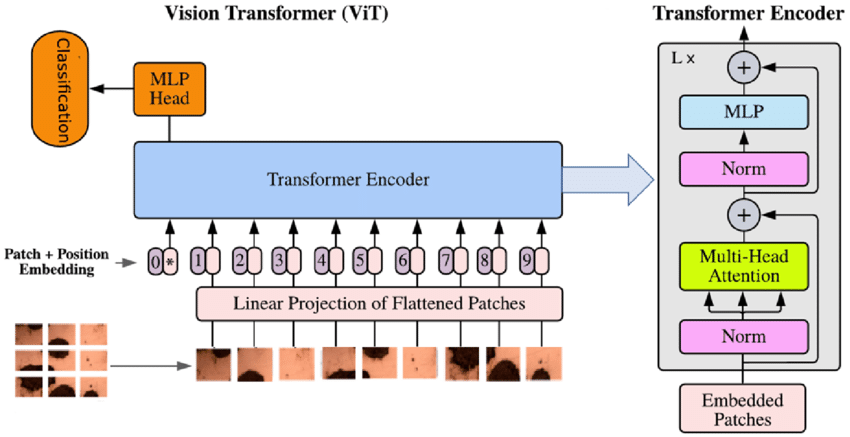
\includegraphics[width=\linewidth]{tikz/chapter8 - Vision Transformer.png}
    \caption{{\color{red}\colorbox{pink}{Tikz TO-DO}} ViT architecture}
\end{figure}

The input (as a patch) is embedded in a smaller size to reduce complexity. In addition, ViT adds an additional learnable embedding called \textbf{class token}, colored gray in the figure above, which is a randomly initialized embedding vector learned during the training process. This is used to collect global information from the image through the Transformer's self-attention mechanism. At the end of the process, the MLP (Multilayer Perceptron) head \textbf{only looks at the data from the class token of the last layer} and no other information.

When trained on medium-sized datasets such as ImageNet, such models show modest accuracies (a few points below ResNets of comparable size). Transformers lack some of the inductive biases present in CNNs, such as translation equivalence and locality, and thus \textbf{do not generalize well when trained on insufficient amounts of data}. However, the situation changes if the models are trained on larger datasets (14M-300M images).

\section{Swin Transformer}

Unlike ViT, which is not optimized for dense recognition tasks, the Swin Transformer can serve as a general skeleton for these tasks as well. Presented in \href{https://arxiv.org/pdf/2103.14030}{"Swin Transformer: Hierarchical Vision Transformer using Shifted Windows" (Hu et al.)}, this model builds hierarchical feature maps by joining image patches in the deepest layers. By using dynamic partitioning, it improves the accuracy of localized representations. 

\begin{figure}[!htbp]
    \centering
    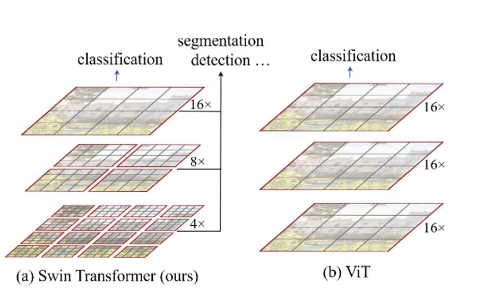
\includegraphics[width=0.85\linewidth]{tikz/chapter8 - Swin Transformer.png}
    \caption{{\color{red}{\colorbox{pink}{Tikz TO-DO}}} Comparison of Swin and ViT}
\end{figure}

The image shows the comparison between Swin Transformer and ViT when calculating self-attention. The Swin calculates self-attention in sub-areas of the image. At each level, the Swin Transformer partitions the image into regular windows and calculates the self-attention within each window. When moving to the next level, the window layout is updated, creating \textbf{new windows that may partially or completely overlap the previous windows}. This approach allows the model to manage and integrate information from different parts of the image effectively, improving its ability to capture complex, long-range relationships.